
% ----------------------------------------------------------------------
%  Set the document class
% ----------------------------------------------------------------------
\documentclass[11pt,a4paper,twoside]{article}

% ----------------------------------------------------------------------
% Define external packages, language, margins, fonts and new commands
% ----------------------------------------------------------------------
%\input{preamble} 
\usepackage[utf8]{inputenc}   % <<<<< Linux
\usepackage[english]{babel} % <<<<< English
\usepackage{notoccite}
\usepackage[skip=0.5\baselineskip]{caption}
\hyphenation{GTKWave}
\usepackage{listings}
\usepackage[all]{nowidow}

\usepackage{listings}

%\usepackage[ascii]{inputenc}
\usepackage{siunitx}
\usepackage{lmodern}
\usepackage[T1]{fontenc}
\usepackage[babel=true]{microtype}




\makeatletter
\newread\pin@file
\newcounter{pinlineno}
\newcommand\pin@accu{}
\newcommand\pin@ext{pintmp}
% inputs #3, selecting only lines #1 to #2 (inclusive)
\newcommand*\partialinput [3] {%
  \IfFileExists{#3}{%
    \openin\pin@file #3
    % skip lines 1 to #1 (exclusive)
    \setcounter{pinlineno}{1}
    \@whilenum\value{pinlineno}<#1 \do{%
      \read\pin@file to\pin@line
      \stepcounter{pinlineno}%
    }
    % prepare reading lines #1 to #2 inclusive
    \addtocounter{pinlineno}{-1}
    \let\pin@accu\empty
    \begingroup
    \endlinechar\newlinechar
    \@whilenum\value{pinlineno}<#2 \do{%
      % use safe catcodes provided by e-TeX's \readline
      \readline\pin@file to\pin@line
      \expandafter\expandafter\expandafter\def\expandafter\expandafter\expandafter\pin@accu\expandafter\expandafter\expandafter{\expandafter\pin@accu\pin@line}
      %\edef\pin@accu{\pin@accu\pin@line}%
      \stepcounter{pinlineno}%
    }
    \closein\pin@file
    \expandafter\endgroup
    \scantokens\expandafter{\pin@accu}%
  }{%
    \errmessage{File `#3' doesn't exist!}%
  }%
}
\makeatother

%blind text
\usepackage{lipsum}

\usepackage{graphicx}
\graphicspath{ {./} {../../figlib/} }
\def\FontLn{% 16 pt normal
  \usefont{T1}{phv}{m}{n}\fontsize{16pt}{16pt}\selectfont}
\def\FontLb{% 16 pt bold
  \usefont{T1}{phv}{b}{n}\fontsize{16pt}{16pt}\selectfont}
\def\FontMn{% 14 pt normal
  \usefont{T1}{phv}{m}{n}\fontsize{14pt}{14pt}\selectfont}
\def\FontMb{% 14 pt bold
  \usefont{T1}{phv}{b}{n}\fontsize{14pt}{14pt}\selectfont}
\def\FontSn{% 12 pt normal
  \usefont{T1}{phv}{m}{n}\fontsize{12pt}{12pt}\selectfont}

% Use Arial font as default
%
\renewcommand{\rmdefault}{phv}
\renewcommand{\sfdefault}{phv}
\usepackage{geometry}	
\geometry{verbose,tmargin=2.5cm,bmargin=2.5cm,lmargin=2.5cm,rmargin=2.5cm}

%\usepackage{setspace}
%\renewcommand{\baselinestretch}{1.5}

\usepackage[pdftex]{hyperref} % enhance documents that are to be
                              % output as HTML and PDF
\hypersetup{colorlinks,       % color text of links and anchors,
                              % eliminates borders around links
%            linkcolor=red,    % color for normal internal links
            linkcolor=black,  % color for normal internal links
            anchorcolor=black,% color for anchor text
%            citecolor=green,  % color for bibliographical citations
            citecolor=black,  % color for bibliographical citations
%            filecolor=magenta,% color for URLs which open local files
            filecolor=black,  % color for URLs which open local files
%            menucolor=red,    % color for Acrobat menu items
            menucolor=black,  % color for Acrobat menu items
%            pagecolor=red,    % color for links to other pages
            pagecolor=black,  % color for links to other pages
%            urlcolor=cyan,    % color for linked URLs
            urlcolor=black,   % color for linked URLs
	          bookmarks=true,         % create PDF bookmarks
	          bookmarksopen=false,    % don't expand bookmarks
	          bookmarksnumbered=true, % number bookmarks
	          pdftitle={report},
            pdfauthor={Andre C. Marta},
%            pdfsubject={Thesis Title},
%            pdfkeywords={Thesis Keywords},
            pdfstartview=FitV,
            pdfdisplaydoctitle=true}

\usepackage[numbers,sort&compress]{natbib} % <<<<< References in numbered list [1],[2],...
\usepackage{subcaption} 
\usepackage{mdframed}

%%%%%%%%%%%%%%%%%%%%%%%%%%%%%%%%%%%%%%%%%%%%%%%%%%%%%%%%%%%%%%%%%%%%%%%%
%     Begin Document                                                   %
%%%%%%%%%%%%%%%%%%%%%%%%%%%%%%%%%%%%%%%%%%%%%%%%%%%%%%%%%%%%%%%%%%%%%%%%


\begin{document}

% Set plain page style (no headers, footer with centered page number)
\pagestyle{plain}

% Set roman numbering (i,ii,...) before the start of chapters
%\pagenumbering{roman}

% ----------------------------------------------------------------------
%  Cover page
% ----------------------------------------------------------------------
%%%%%%%%%%%%%%%%%%%%%%%%%%%%%%%%%%%%%%%%%%%%%%%%%%%%%%%%%%%%%%%%%%%%%%%%
%                                                                      %
%     File: Thesis_FrontCover.tex                                      %
%     Tex Master: Thesis.tex                                           %
%                                                                      %
%     Author: Andre C. Marta                                           %
%     Last modified :  2 Jul 2015                                      %
%                                                                      %
%%%%%%%%%%%%%%%%%%%%%%%%%%%%%%%%%%%%%%%%%%%%%%%%%%%%%%%%%%%%%%%%%%%%%%%%

\thispagestyle {empty}

% IST Logo - Signature A
% parameters: bb=llx lly urx ury (bounding box), width=h_length, height=v_length, angle=angle, scale=factor, clip=true/false, draft=true/false. 
\includegraphics[bb=9.5cm 11cm 0cm 0cm,scale=0.29]{IST_A_CMYK_POS}

\begin{center}
%
% Figure (Image or plot)
\vspace{1.0cm}
% height = 50 mm
%\includegraphics[height=50mm]{Figures/Airbus_A350.jpg}

% Title, author and degree
\vspace{1cm}
{\FontLb Circuit Theory and Electronics Fundamentals} \\ % <<<<< EDIT TITLE
\vspace{1cm}
{\FontSn Integrated Master in Aerospace Engineering, Técnico, University of Lisbon} \\ % <<<<< EDIT COURSE
\vspace{1cm}
{\FontSn Lab4: Audio Amplifier circuit} \\
\vspace{1cm}
{\FontSn May 23, 2021} \\ % <<<<< EDIT DATE (corresponds to date of oral examination)
\vspace{1cm}
{\FontSn Jo\~{a}o Maria Mendes, 95804 \\ Maria Magalh\~{a}es, 95825 \\ Mariana Afonso, 95827}
 
%
\end{center}



% ----------------------------------------------------------------------
% Dedication page (optional)
% ----------------------------------------------------------------------
%\input{dedication} 
%\cleardoublepage

% ----------------------------------------------------------------------
%  Acknowledgments (optional)
% ----------------------------------------------------------------------
%\input{acknowledgements}
%\cleardoublepage

% ----------------------------------------------------------------------
%  Abstract (both in English and Portuguese)
% ----------------------------------------------------------------------
%\input{resumo} 
%\cleardoublepage

%\input{abstract} 

% ----------------------------------------------------------------------
%  Table of contents, list of tables, list of figures and nomenclature
% ----------------------------------------------------------------------

% Table of contents
%
\tableofcontents

% List of tables
%\addcontentsline{toc}{section}{\listtablename}
%\listoftables
%\cleardoublepage 

% List of figures
%\addcontentsline{toc}{section}{\listfigurename}
%\listoffigures
%\cleardoublepage 

% Set arabic numbering (1,2,...) after preface
%
%\setcounter{page}{1}
%\pagenumbering{arabic}

% ----------------------------------------------------------------------
%  Body
% ----------------------------------------------------------------------

\newpage
\section{Introduction}
\label{sec:introduction}

%state the learning objective 
The objective of this laboratory assignment is to build a bandpass filter with a central frequency of 1kHz and a gain of 40dB.
The circuit created and analysed in this assignment can be seen in Figure~\ref{fig:Circuit}.\\
\noindent In order to evaluate how successfully our goal has been achieved, we calculate the merit M of our work, using the following expression:
\begin{equation}
M = \frac{1}{cost(*GainDeviation*CentralFreqDeviation + 10^{-6})}
  \label{eq:merit}
\end{equation}
where the cost is given by cost = cost of resistors + cost of capacitors + cost of transistors, knowing that each kOhm costs 1 monetary unit (MU), 
each $\mu$F costs 1 MU and each transistor costs 0,1 MU.
\noindent In Section~\ref{sec:analysis}, a theoretical analysis of the circuit is
presented, using Octave. In Section~\ref{sec:simulation}, the circuit is analysed by
simulation using ngspice. The conclusions of this study are outlined in
Section~\ref{sec:conclusion}. In addiction, the results are compared to the theoretical results obtained in Section~\ref{sec:analysis}.

\begin{figure}[h!] \centering
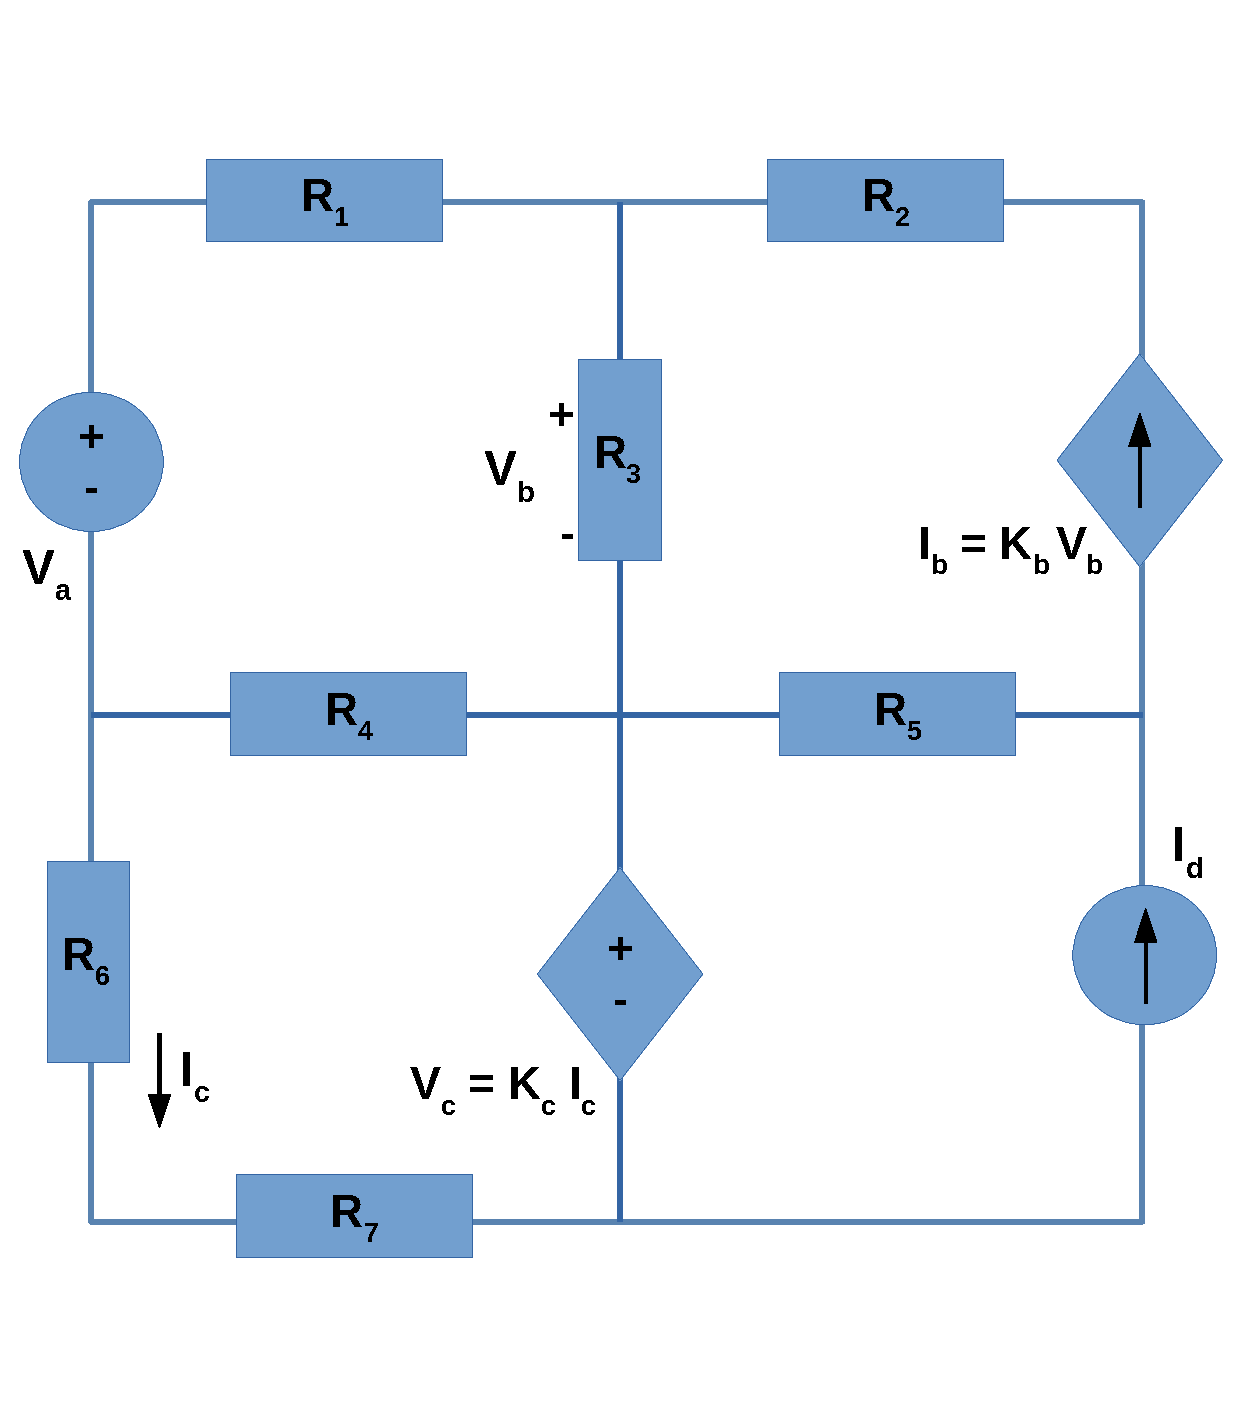
\includegraphics[width=1\linewidth]{Circuit.pdf}
\caption{Circuit analysed.}
\label{fig:Circuit}
\end{figure}



\newpage
\section{Theoretical Analysis}
\label{sec:analysis}
In this section, the circuit shown in Figure~\ref{fig:Circuit} is analysed
theoretically, using the mesh method and the node method. \\
In the first one, we define a current for each elementary mesh, 
which is a loop containing no other loops, with an arbitrary direction.
These currents will be our unknown values and the objetive is to compute them, using the Ohm's Law (V = RI) and Kirchhoff Voltage Law. 
Therefore, in this circuit we wil have four currents to compute, so we have to find four equations to solve this problem. \\
\noindent In the second one, each circuit node have a defined voltage. We also choose a node to have a null voltage.
Then, we use Ohm's Law and Kirchhoff Current Law in nodes that are not connected to a voltage source.
In the end, we write additional equations for the nodes related by voltage sources.
Consequently, we will have an equal number of nodes and equations.
To calculate the unkown voltages and currents, we use the following values (Resistances in kOhm, voltages in Volts, capacity in F, $K_b$ in S and $K_d$ in Ohms):
\begin{table}[h!]
\centering
\begin{small}
\caption{Given values by Python.} \label{Table1}
\begin{tabular}{|c|c|}
\hline
$R_1$ & 1,00332071212 \\
$R_2$  & 2,04460853047 \\
$R_3$  & 3,08291730437 \\
$R_4$ & 4,16061678649 \\
$R_5$  & 3,04022345043 \\
$R_6$ & 2,06711403452 \\
$R_7$ & 1,03302701196 \\
$V_s$ & 5,13988034104\\
$C$ & 1,02475824097e-06 \\
$K_b$ & 7,0544535009e-03 \\
$K_c$ & 8,16113797582e+03\\
\hline
\end{tabular}
\end{small}
\end{table}

\newpage

\section{Mesh method}

\noindent In Figure~\ref{fig:Circuit_Mesh}, we defined a current for each circuit essencial loop.
As said before, we will have four equations, because we need to compute four currents
($I_1$, $I_2$, $I_3$ and $I_4$).
In this analysis, we assumed that the current in mesh one is flowing clockwise and the three other currents are flowing in the other direction. Once we calculate the values to each current with the KVL method, we know that the negative ones are not flowing in the direction we assumed.

\noindent Starting with mesh 3, we can see by inspection that $I_c$ = $I_3$  and that $R_3$  depends on $I_1$  and $I_3$, which have the same direction. The other 3 components depend only on $I_3$. In the voltage source, the current flows to the positive side to the negative, so it is not aligned with the direction we selected. Hence, we must consider it negative. So we have this equation:
\begin{equation}
(I_3 + I_1)R_4 + I_3R_7+I_3R_6 - K_cI_3  = 0
  \label{eq:kcl_mesh3}
\end{equation}

\noindent In circuit analysis, we always consider the current flowing from the negative side to the positive, so in mesh 1, the voltage source is not aligned with the selected direction. For that reason, we consider $V_a$ negative. The current in $R_1$ depends only in $I_1$, which we can see by inspection, and $R_3$  and $R_4$  depend on two different currents with the same direction, which is positive because we assumed the clockwise direction. So we have: 
\begin{equation}
(I_1 + I_3)R_4 - V_a + R_3(I_2 + I_1)+ R_1I_1 = 0
  \label{eq:kcl_mesh1}
\end{equation}

\noindent We already have two equations, but we are going to need two additional ones, since we can not use this method in meshes with current sources. We can get these two equations by inspection of the two current sources. Starting with the dependent source $I_b$, we already  know the relation between this source and $V_b$, so we only have to write this term as a function of resistances and currents. We already wrote $V_b$ as a function of $R_3$, $I_2$ and $I_1$ at the third term of the previous equation for mesh 1. So we write it again:
\begin{equation}
I_2 = K_bR_3(I_2+I_1)
  \label{eq:kcl_mesh2}
\end{equation}

\noindent Finishing with the simplest equation, we can look at the fourth mesh to verify that:
\begin{equation}
I_4 = I_d
  \label{eq:kvl_kcl_mesh4}
\end{equation}

\noindent All these equations can be transformed in a matricial system as it is shown here:
$$ \left[ \begin{array}{cccc} R_4 & 0 & R_6 + R_4 + R_7- K_c  & 0\\
R_4 + R_3 + R_1   & R_3  &  R_4  & 0 \\
K_bR_3 & -1 + K_bR_3 & 0 & 0 \\
 0 & 0 & 0 & 1 \end{array} \right]
\left[ \begin{array}{c} I_1 \\ I_2 \\ I_3 \\ I_4\end{array} \right] = 
\left[ \begin{array}{c} 0 \\ V_a \\ 0 \\ I_d \end{array} \right] $$

\noindent Solving this system using Octave and the values given, we have obtained this values:
\begin{table}[h!]
\centering
\begin{small}
\caption{Meshes table.} \label{Table2}
\begin{tabular}{|c|c|}
\hline
Meshes currents & Values obtained (Ampers)\\
\hline
$I_1$ & \partialinput{1}{1}{tabelaM.tex} \\
$I_2$  & \partialinput{2}{2}{tabelaM.tex} \\
$I_3$  & \partialinput{3}{3}{tabelaM.tex}\\
$I_4$   & \partialinput{4}{4}{tabelaM.tex} \\
\hline
\end{tabular}
\end{small}
\end{table}

\noindent With this currents, we can discover node voltages and currents passing through each resistance, with the following equations, and knowing that $V_c$ = $K_c$$I_3$:

\begin{equation}
I_ b = I_2
  \label{eq: IB}
\end{equation}

\begin{equation}
I_ d = I_4
  \label{eq: I4}
\end{equation}

\begin{equation}
R_1[i] = I_1
  \label{eq: IR1}
\end{equation}

\begin{equation}
R_2[i] = I_2
  \label{eq: IR2}
\end{equation}

\begin{equation}
R_3[i] = I_1 + I_2
  \label{eq: IR3}
\end{equation}

\begin{equation}
R_4[i] = I_1 + I_3
  \label{eq: IR4}
\end{equation}

\begin{equation}
R_5[i] = I_4 - I_2
  \label{eq: IR5}
\end{equation}

\begin{equation}
R_6[i] = I_3
  \label{eq: IR6}
\end{equation}

\begin{equation}
R_7[i] = I_3
  \label{eq: IR7}
\end{equation}

\begin{equation}
V_b = \frac{I_b}{K_b}
  \label{eq: Vb}
\end{equation}

\begin{equation}
V_7 = V_c
  \label{eq: V7}
\end{equation}

\begin{equation}
V_6 = V_b + V_7
\label{eq: V6}
\end{equation}

\begin{equation}
V_5 = V_6 + R_2I_2
  \label{eq: V5}
\end{equation}

\begin{equation}
V_4 = V_7 + R_5(I_4 - I_2)
  \label{eq: V4}
\end{equation}

\begin{equation}
V_3 = R_7I_3
  \label{eq: V3}
\end{equation}

\begin{equation}
V_2 = V_3 + R_6I_3
  \label{eq: V2}
\end{equation}

\begin{equation}
V_1 = V_2 + V_a
\label{eq: V1}
\end{equation}

Voltage values, represented by $V_i$, are given in Volts and currents, represented by $I_i$ or $R_i$[i] in Ampers.
\begin{table}[h!]
\centering
\begin{small}
\caption{Currents and voltages obtained by mesh method.} \label{Table3}
\begin{tabular}{|c|c|}
\hline
Meshes currents & Values obtained (Ampers/Volts)\\
\hline
$I_b$ & \partialinput{1}{1}{tabelaM2.tex} \\
$I_d$  & \partialinput{2}{2}{tabelaM2.tex} \\
$R_1[i]$  & \partialinput{3}{3}{tabelaM2.tex}\\
$R_2[i]$   & \partialinput{4}{4}{tabelaM2.tex} \\
$R_3[i]$ & \partialinput{5}{5}{tabelaM2.tex} \\
$R_4[i]$  & \partialinput{6}{6}{tabelaM2.tex} \\
$R_5[i]$ & \partialinput{7}{7}{tabelaM2.tex}\\
$R_6[i]$   & \partialinput{8}{8}{tabelaM2.tex} \\
$R_7[i]$ & \partialinput{9}{9}{tabelaM2.tex} \\
$V_1$  & \partialinput{10}{10}{tabelaM2.tex} \\
$V_2$  & \partialinput{11}{11}{tabelaM2.tex}\\
$V_3$   & \partialinput{12}{12}{tabelaM2.tex} \\
$V_4$  & \partialinput{13}{13}{tabelaM2.tex} \\
$V_5$  & \partialinput{14}{14}{tabelaM2.tex}\\
$V_6$   & \partialinput{15}{15}{tabelaM2.tex} \\
$V_7$   & \partialinput{16}{16}{tabelaM2.tex} \\
\hline
\end{tabular}
\end{small}
\end{table}

\newpage
\section{Node method}
\noindent In Figure~\ref{fig:Circuit_Nodes}, we defined a voltage for each circuit node and a node with null voltage.
As said before, we will have seven equations, because we need to compute seven voltages 
($V_1$, $V_2$, $V_3$, $V_4$, $V_5$, $V_6$ and $V_7$).
In this analysis, we consider currents diverging from the node as positive values and currents converging as negative values, using KCL.

\noindent Starting with node 3, for this node, we considered all currents diverging, so we have this equation:
\begin{equation}
\frac{V_3 - V_2}{R_6} + \frac{V_3}{R_7} = 0
  \label{eq:kvl_node3}
\end{equation}

\noindent In node 4, only $I_d$ is converging.
$V_B$ is equal to $V_6$ - $V_7$, due to the direction represented in the circuit for $R_3$ voltage:
\begin{equation}
\frac{V_4 - V_7}{R_5} - I_d + K_b(V_6 - V_7) = 0
  \label{eq:kvl_node4}
\end{equation}

\noindent Moving on to node 5, in which only $I_b$ is converging, having this equation:
\begin{equation}
\frac{V_5 - V_6}{R_2} - K_b(V_6 - V_7) = 0
  \label{eq:kvl_node5}
\end{equation}

\noindent On the other side, in node 6, we considered all currents diverging:
\begin{equation}
\frac{V_6 - V_7}{R_3} + \frac{V_6 - V_5}{R_2} + \frac{V_6 - V_1}{R_1} = 0
  \label{eq:kvl_node6}
\end{equation}

\noindent The next equation establish the relation between nodes 1 and 2 voltages:
\begin{equation}
V_1 - V_2 = V_a
  \label{eq:kvl_node12}
\end{equation}

\noindent The relation between GND and node 7 is showed in the next equation:
\begin{equation}
V_7 = \frac{K_c(V_2 - V_3)}{R_6}
  \label{eq:kvl_node7GND}
\end{equation}

\noindent Since there is still an equation missing, we considered a super node containing $V_a$ and $R_6$ and all currents diverging:
\begin{equation}
\frac{V_1 - V_6}{R_1} + \frac{V_2 - V_7}{R_4} + \frac{V_3}{R_7} = 0
  \label{eq:kvl_supernode}
\end{equation}

\noindent All this equations can be transformed in a matricial system as it is showed here:
$$ \left[ \begin{array}{ccccccc} 0 & -\frac{1}{R_6} & \frac{1}{R_6} + \frac{1}{R_7} & 0 & 0 & 0 & 0 \\
0 & 0 & 0 & \frac{1}{R_5} & 0 & K_b & -K_b - \frac{1}{R_5} \\
0 & 0 & 0 & 0 & \frac{1}{R_2} & -K_b - \frac{1}{R_2} & K_b
\\ -\frac{1}{R_1} & 0 & 0 & 0 & -\frac{1}{R_2} & \frac{1}{R_1} + \frac{1}{R_2} + \frac{1}{R_3} & -\frac{1}{R_3}
\\ 1 & -1 & 0 & 0 & 0 & 0 & 0
\\ 0 & \frac{K_c}{R_6} & -\frac{K_c}{R_6} & 0 & 0 & 0 & -1
\\ \frac{1}{R_1} & \frac{1}{R_4} & \frac{1}{R_7} & 0 & 0 & -\frac{1}{R_1} & -\frac{1}{R_4}\end{array} \right]
\left[ \begin{array}{c} V_1 \\ V_2 \\ V_3 \\ V_4 \\ V_5 \\ V_6 \\ V_7\end{array} \right] = 
\left[ \begin{array}{c} 0 \\ I_d \\ 0 \\ 0 \\ V_a \\ 0 \\ 0\end{array} \right] $$

\noindent Solving this system using Ocatve and the values given, we have obtained this values:
\begin{table}[h!]
\centering
\begin{small}
\caption{Nodes table.} \label{Table4}
\begin{tabular}{|c|c|}
\hline
Nodes Voltages & Values obtained (Volts)\\
\hline
$V_1$           & \partialinput{1}{1}{tabelaV.tex} \\
$V_2$  & \partialinput{2}{2}{tabelaV.tex}\\
$V_3$   &      \partialinput{3}{3}{tabelaV.tex} \\
$V_4$   & \partialinput{4}{4}{tabelaV.tex} \\
$V_5$              & \partialinput{5}{5}{tabelaV.tex} \\
$V_6$     & \partialinput{6}{6}{tabelaV.tex} \\
$V_7$     &  \partialinput{7}{7}{tabelaV.tex}\\
\hline
\end{tabular}
\end{small}
\end{table}

\noindent Having discovered nodes voltages, we need now to obtain the currents flowing in each resistance and $I_b$, with the following equations:

\begin{equation}
I_b = K_b(V_6 - V_7)
  \label{eq:Ib}
\end{equation}

\begin{equation}
R_1[i] = \frac{(V_6 - V_1)}{R_1}
  \label{eq: iR1}
\end{equation}

\begin{equation}
R_2[i] = \frac{(V_5 - V_6)}{R_2}
  \label{eq: iR2}
\end{equation}

\begin{equation}
R_3[i] = \frac{(V_6 - V_7)}{R_3}
  \label{eq: iR3}
\end{equation}

\begin{equation}
R_4[i] = \frac{(V_2 - V_7)}{R_4}
  \label{eq: iR4}
\end{equation}

\begin{equation}
R_5[i] = \frac{(V_4 - V_7)}{R_5}
  \label{eq: iR5}
\end{equation}

\begin{equation}
R_6[i] = \frac{(V_2 - V_3)}{R_6}
  \label{eq: iR6}
\end{equation}

\begin{equation}
R_7[i] = \frac{V_3}{R_7}
  \label{eq: iR7}
\end{equation}

\begin{table}[h!]
\centering
\begin{small}
\caption{Branch currents obtained by node method.} \label{Table5}
\begin{tabular}{|c|c|}
\hline
Branch currents & Values obtained (Ampers)\\
\hline
$I_b$ & \partialinput{1}{1}{tabelaV2.tex} \\
$R_1[i]$  & \partialinput{2}{2}{tabelaV2.tex}\\
$R_2[i]$   & \partialinput{3}{3}{tabelaV2.tex} \\
$R_3[i]$ & \partialinput{4}{4}{tabelaV2.tex} \\
$R_4[i]$  & \partialinput{5}{5}{tabelaV2.tex} \\
$R_5[i]$ & \partialinput{6}{6}{tabelaV2.tex}\\
$R_6[i]$   & \partialinput{7}{7}{tabelaV2.tex} \\
$R_7[i]$ & \partialinput{8}{8}{tabelaV2.tex} \\
\hline
\end{tabular}
\end{small}
\end{table}




\newpage
\section{Simulation Analysis}
\label{sec:simulation}
\subsection{Simulation for t < 0}
\noindent
The first part of this section covers the simulation of the circuit in ngspice for t < 0.
The values obtained, by ngspice, for currents flowing in each resistance or capacitor(Ampers) and nodes voltages (Volts) are showed in the following table:
\begin{table}[h!]
  \centering
  \begin{tabular}{|c|c|}
    \hline    
    {\bf Name} & {\bf Value [A or V]} \\ \hline
    @cb[i] & 0.000000e+00\\ \hline
@ce[i] & 0.000000e+00\\ \hline
@q1[ib] & 7.022567e-05\\ \hline
@q1[ic] & 1.404513e-02\\ \hline
@q1[ie] & -1.41154e-02\\ \hline
@q1[is] & 5.765392e-12\\ \hline
@rc[i] & 1.411536e-02\\ \hline
@re[i] & 1.411536e-02\\ \hline
@rf[i] & 7.022567e-05\\ \hline
@rs[i] & 0.000000e+00\\ \hline
v(1) & 0.000000e+00\\ \hline
v(2) & 0.000000e+00\\ \hline
base & 2.254108e+00\\ \hline
coll & 5.765392e+00\\ \hline
emit & 1.411536e+00\\ \hline
vcc & 1.000000e+01\\ \hline

  \end{tabular}
  \caption{Operating point. A variable preceded by @ is of type {\em current}
    and expressed in Ampere; other variables are of type {\it voltage} and expressed in
    Volt. (g in "gib" refers to the Ngspice notation of a current source controlled by a voltage).}
  \label{tab:op}
\end{table}

\newpage
\subsection{Simulation for t = 0}
The second section covers the simulation of the circuit for t = 0, where the capacitor is replaced with a voltage source, $v_c$ = V(6) - V(8) (V(6) and V(8) are the values obtained in the previous section). This happens because the voltage of the capacitor ($v_c$) when t < 0 is the same when t = 0. However, V(6) and V(8) are not necessarily the same. Therefore, the capacitor is replaced with the voltage source (initial voltage of the capacitor) so that the boundary conditions V(6) and V(8) can be obtained.
\begin{table}[h!]
  \centering
  \begin{tabular}{|c|c|}
    \hline    
    {\bf Name} & {\bf Value [A or V]} \\ \hline
    zout & 7.866317e+00\\ \hline

  \end{tabular}
  \caption{Operating point. A variable preceded by @ is of type {\em current}
    and expressed in Ampere; other variables are of type {\it voltage} and expressed in
    Volt. (g in "gib" refers to the Ngspice notation of a current source controlled by a voltage).}
  \label{tab:op2}
\end{table}
\newpage
\subsection{Natural response simulation}
The third section covers the simulation of the natural response of the circuit in the interval [0;20] ms, using the boundary conditions obtained in the second section (V(6) and V(8)).
\begin{figure}[h!] \centering
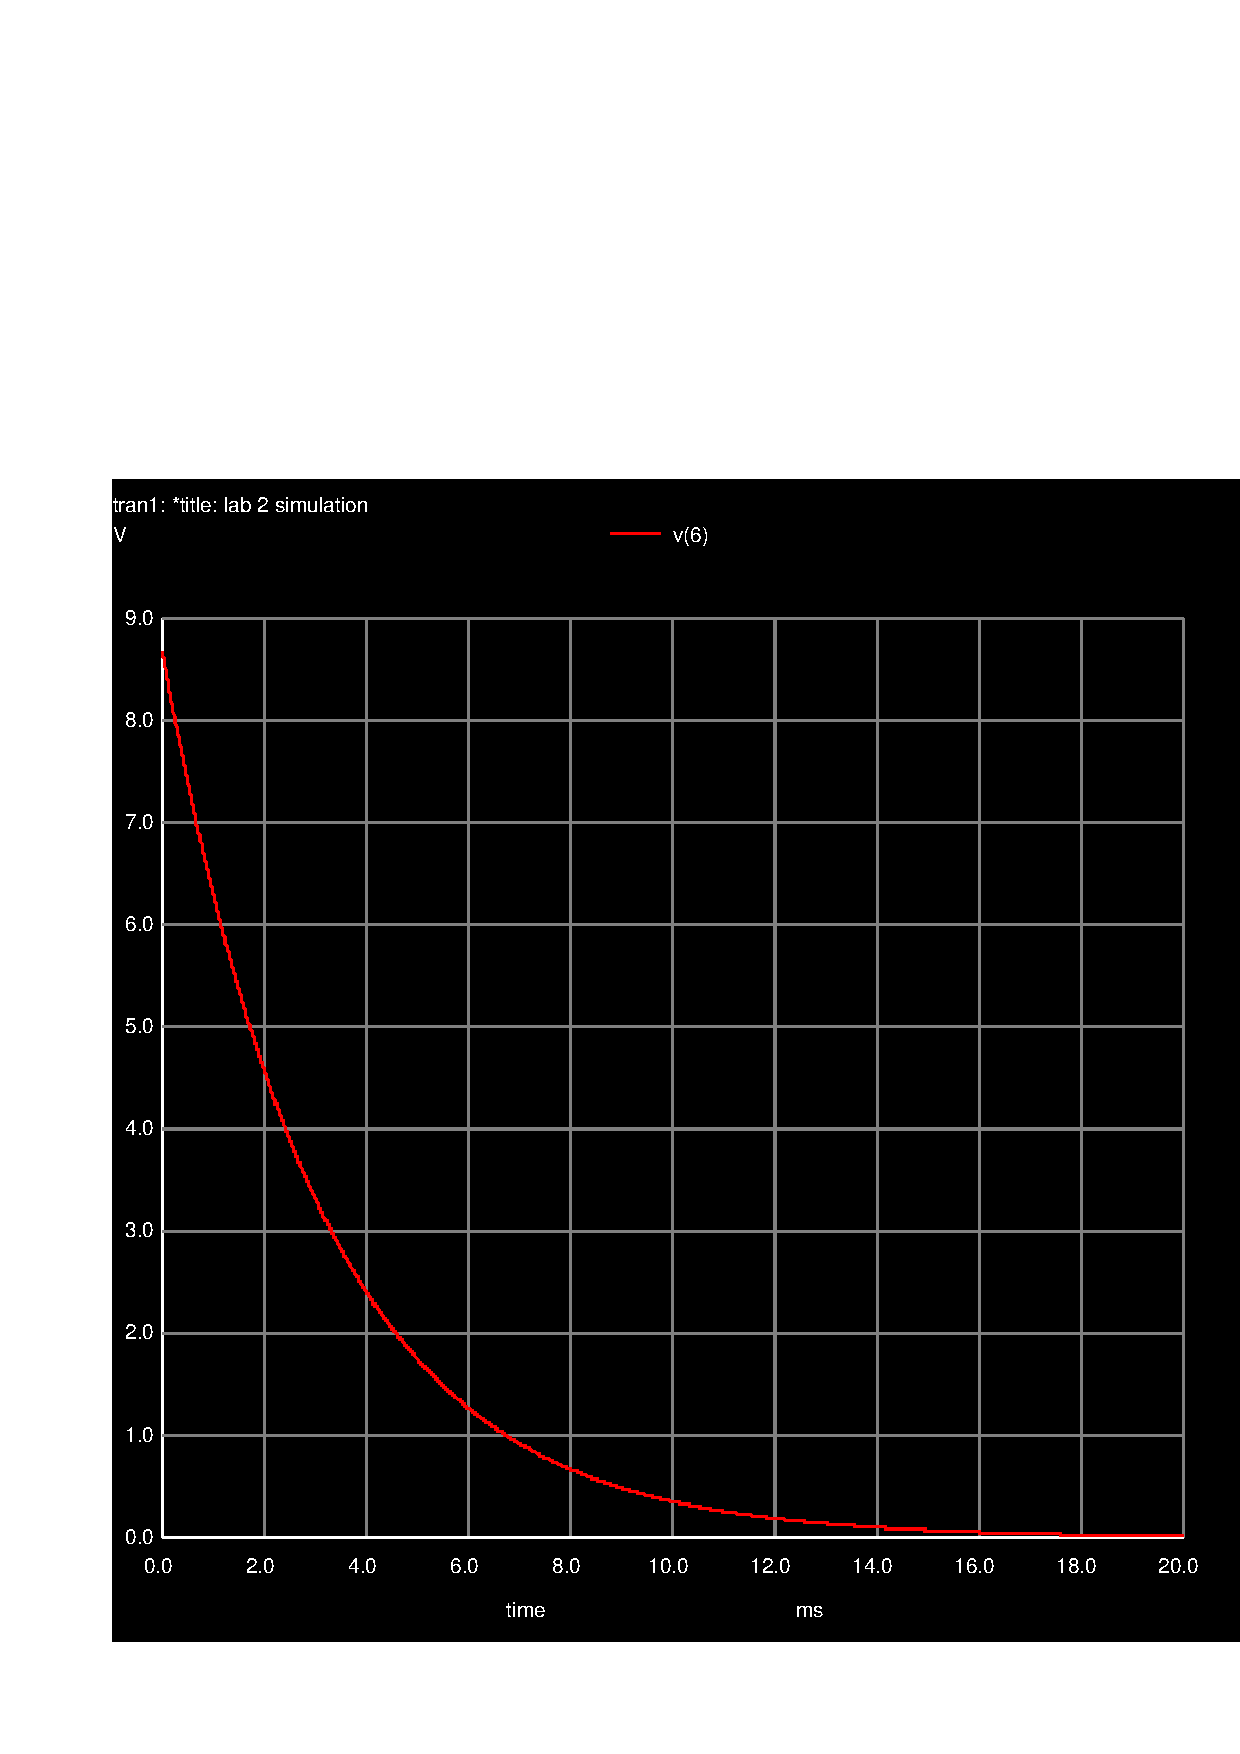
\includegraphics[width=7cm]{../sim/trans.pdf}
\caption{Natural response of $v_6$.}
\label{fig:trans}
\end{figure}
\newpage
\subsection{Total response simulation}
In the forth section, the total response (natural and forced response) is simulated on node 6 in the same interval as the third section, with a given frequency f = 1kHz.
\begin{figure}[h!] \centering
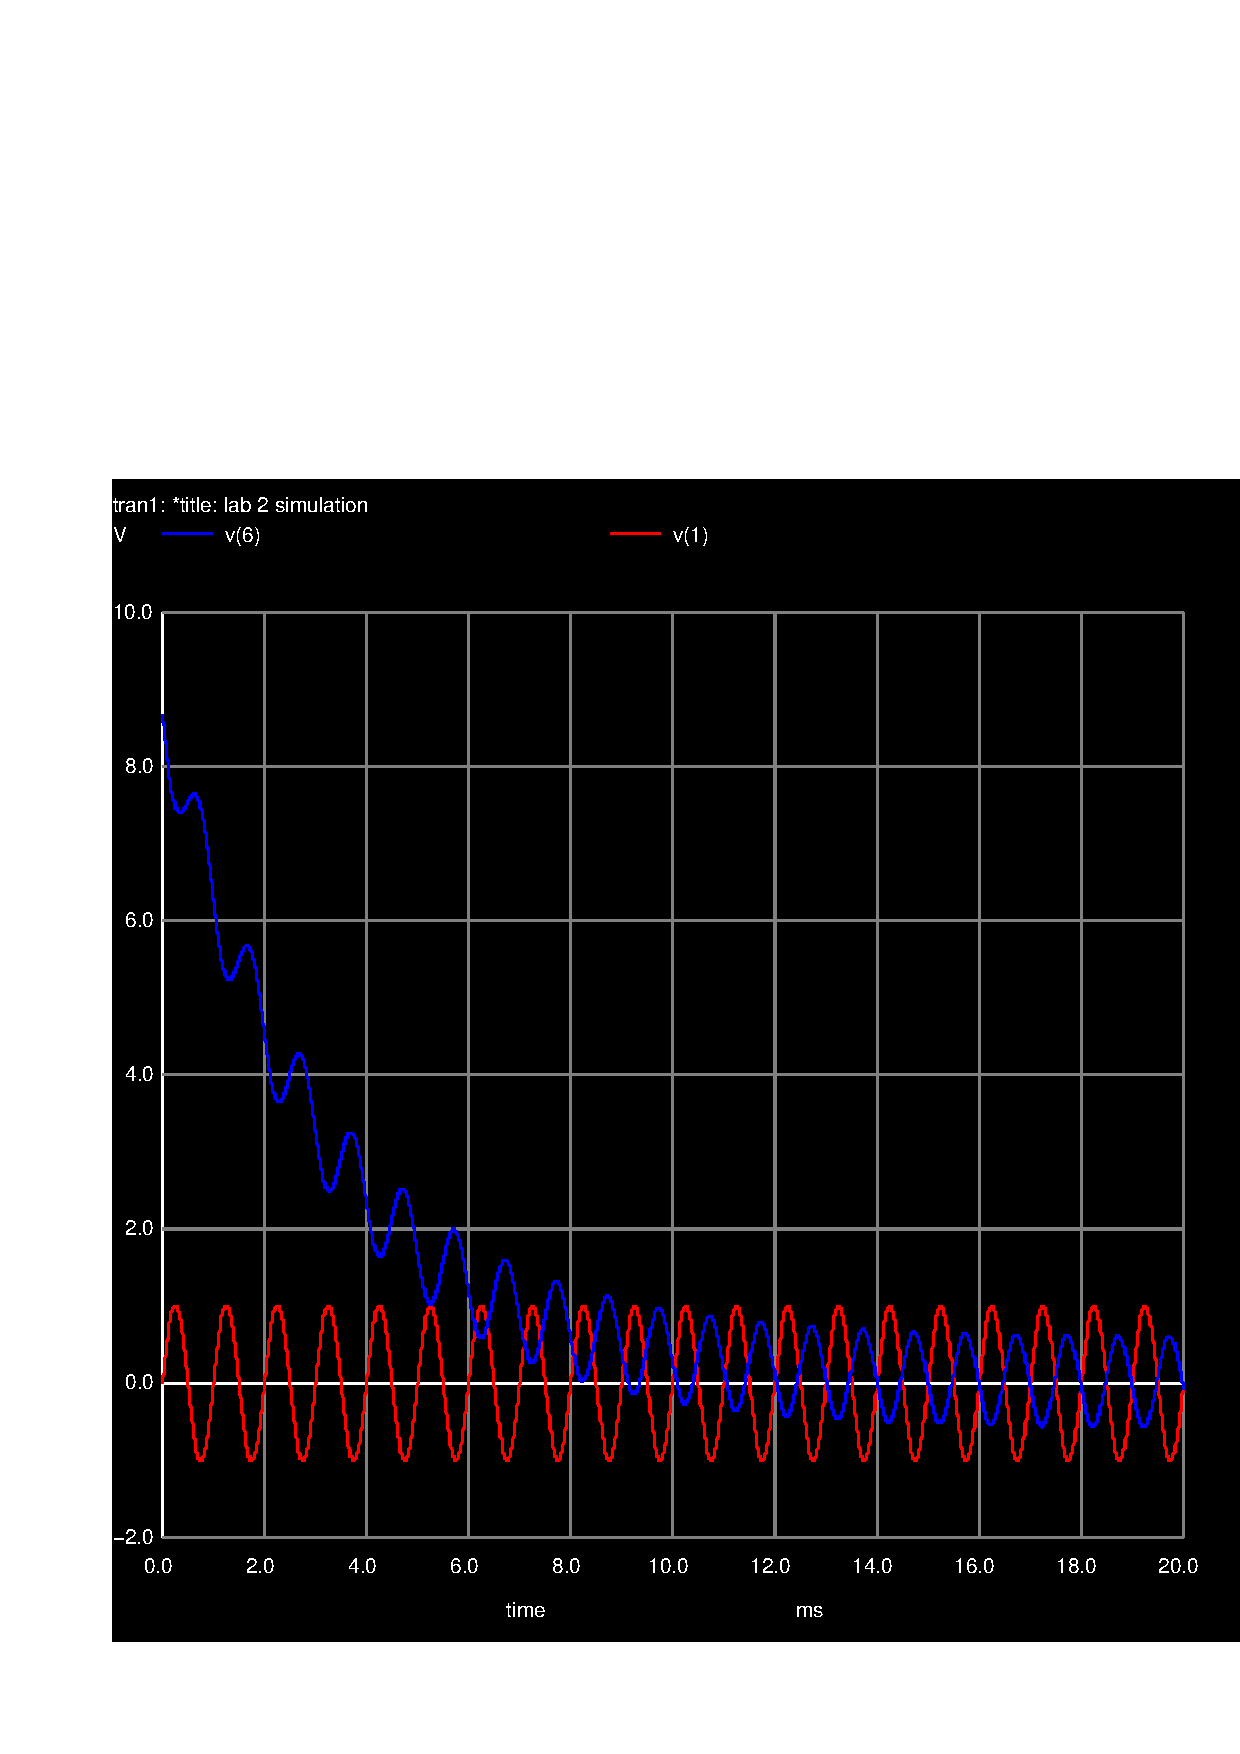
\includegraphics[width=7cm]{../sim/trans2.pdf}
\caption{Total response of $v_6$ and $v_s$.}
\label{fig:trans2}
\end{figure}
\newpage
\subsection{Total response simulation}
In the fifth section, the frequency response is simulated on node 6 (frequency log scale with magnitude in dB, phase in degrees) for the frequency range 0.1 Hz to 1 MHz. The results show that $v_s$(f) stays constant, whereas $v_6$(f) is monotonically decreasing (it decreases 180 degrees in the phase graph and aproximately 6 dB in the magnitude graph). These results derivate from the fact that $v_s$ is the source of the frequency (it will be zero for magnitude graph and 90 for the phase graph) and $v_6$ is an output voltage that is dependent on the frequency source $v_s$.

\begin{figure}[h!] \centering
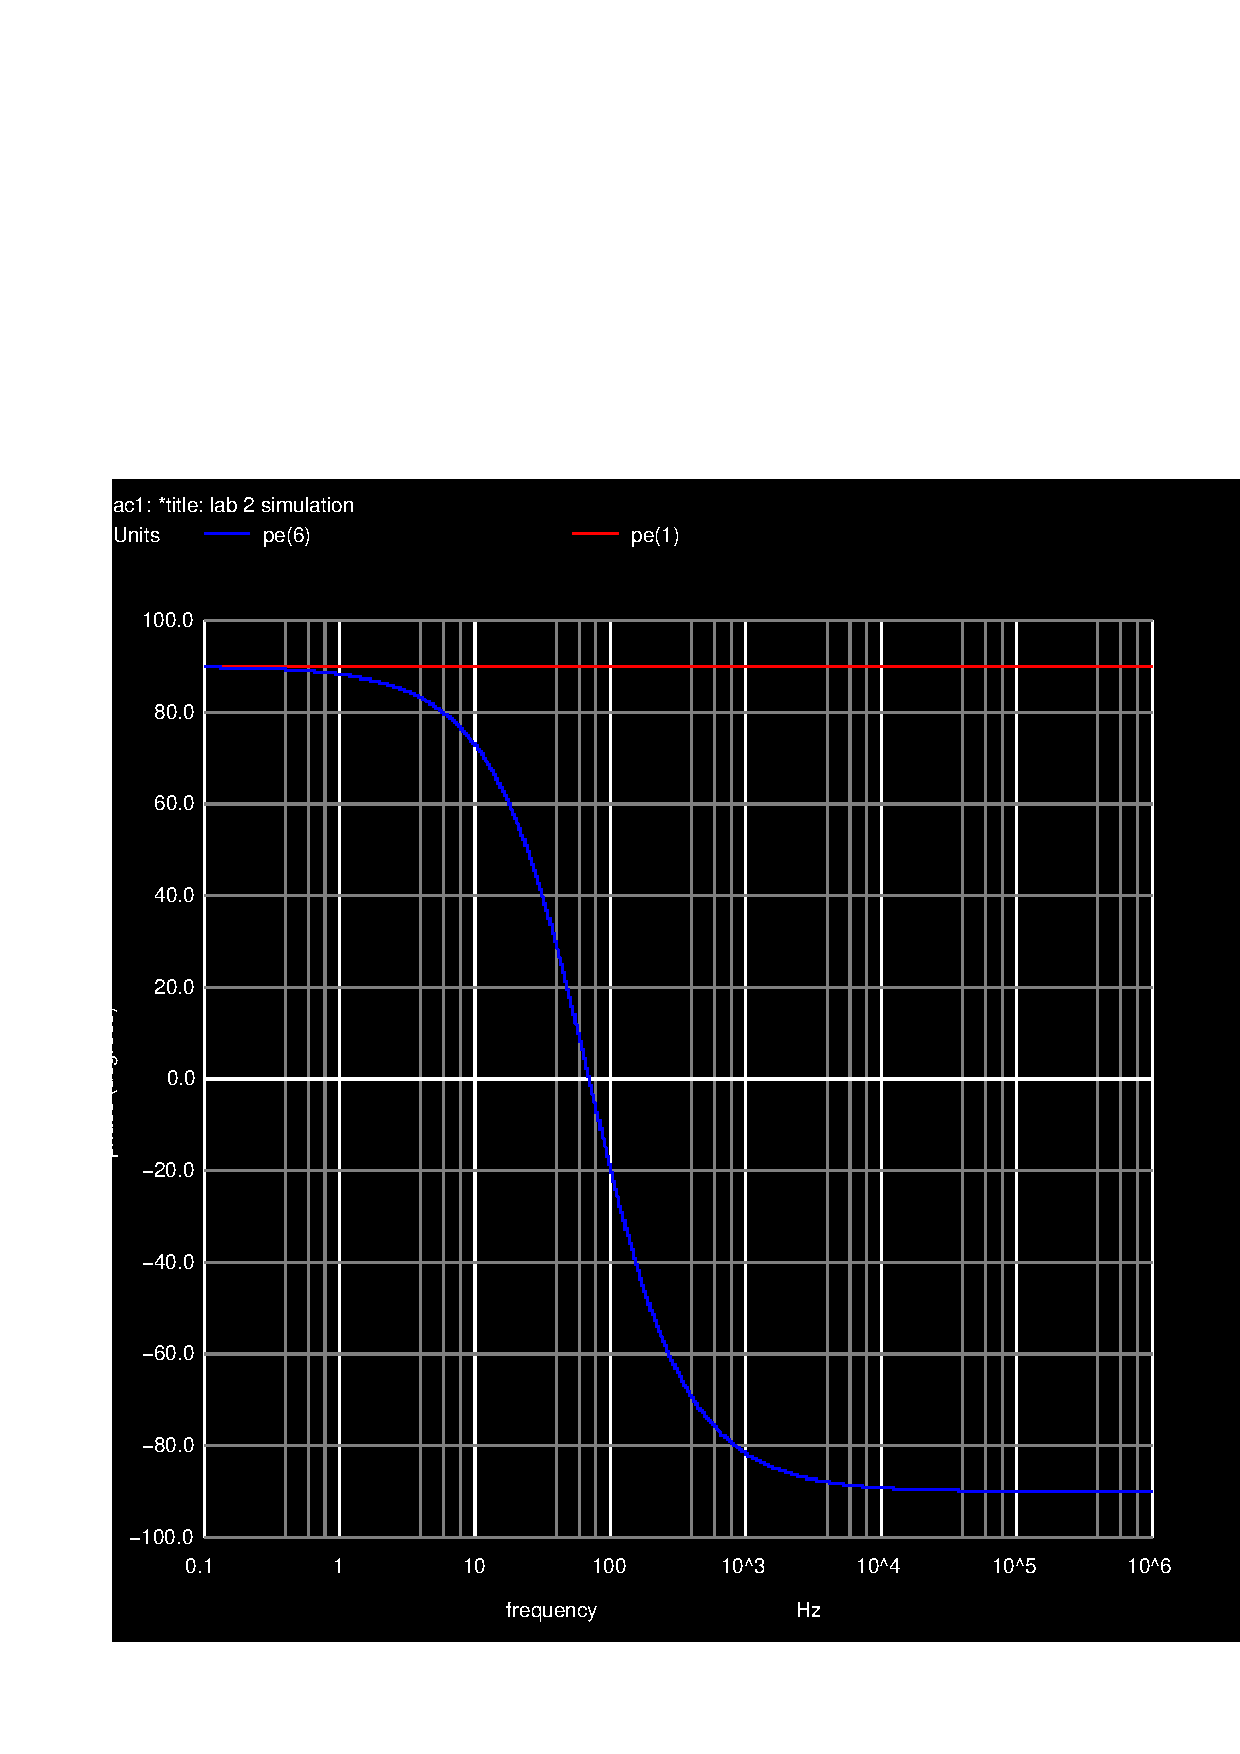
\includegraphics[width=8cm]{../sim/acp.pdf}
\caption{Phase graph for $v_6$ and $v_s$.}
\label{fig:phase}
\end{figure}

\begin{figure}[h!] \centering
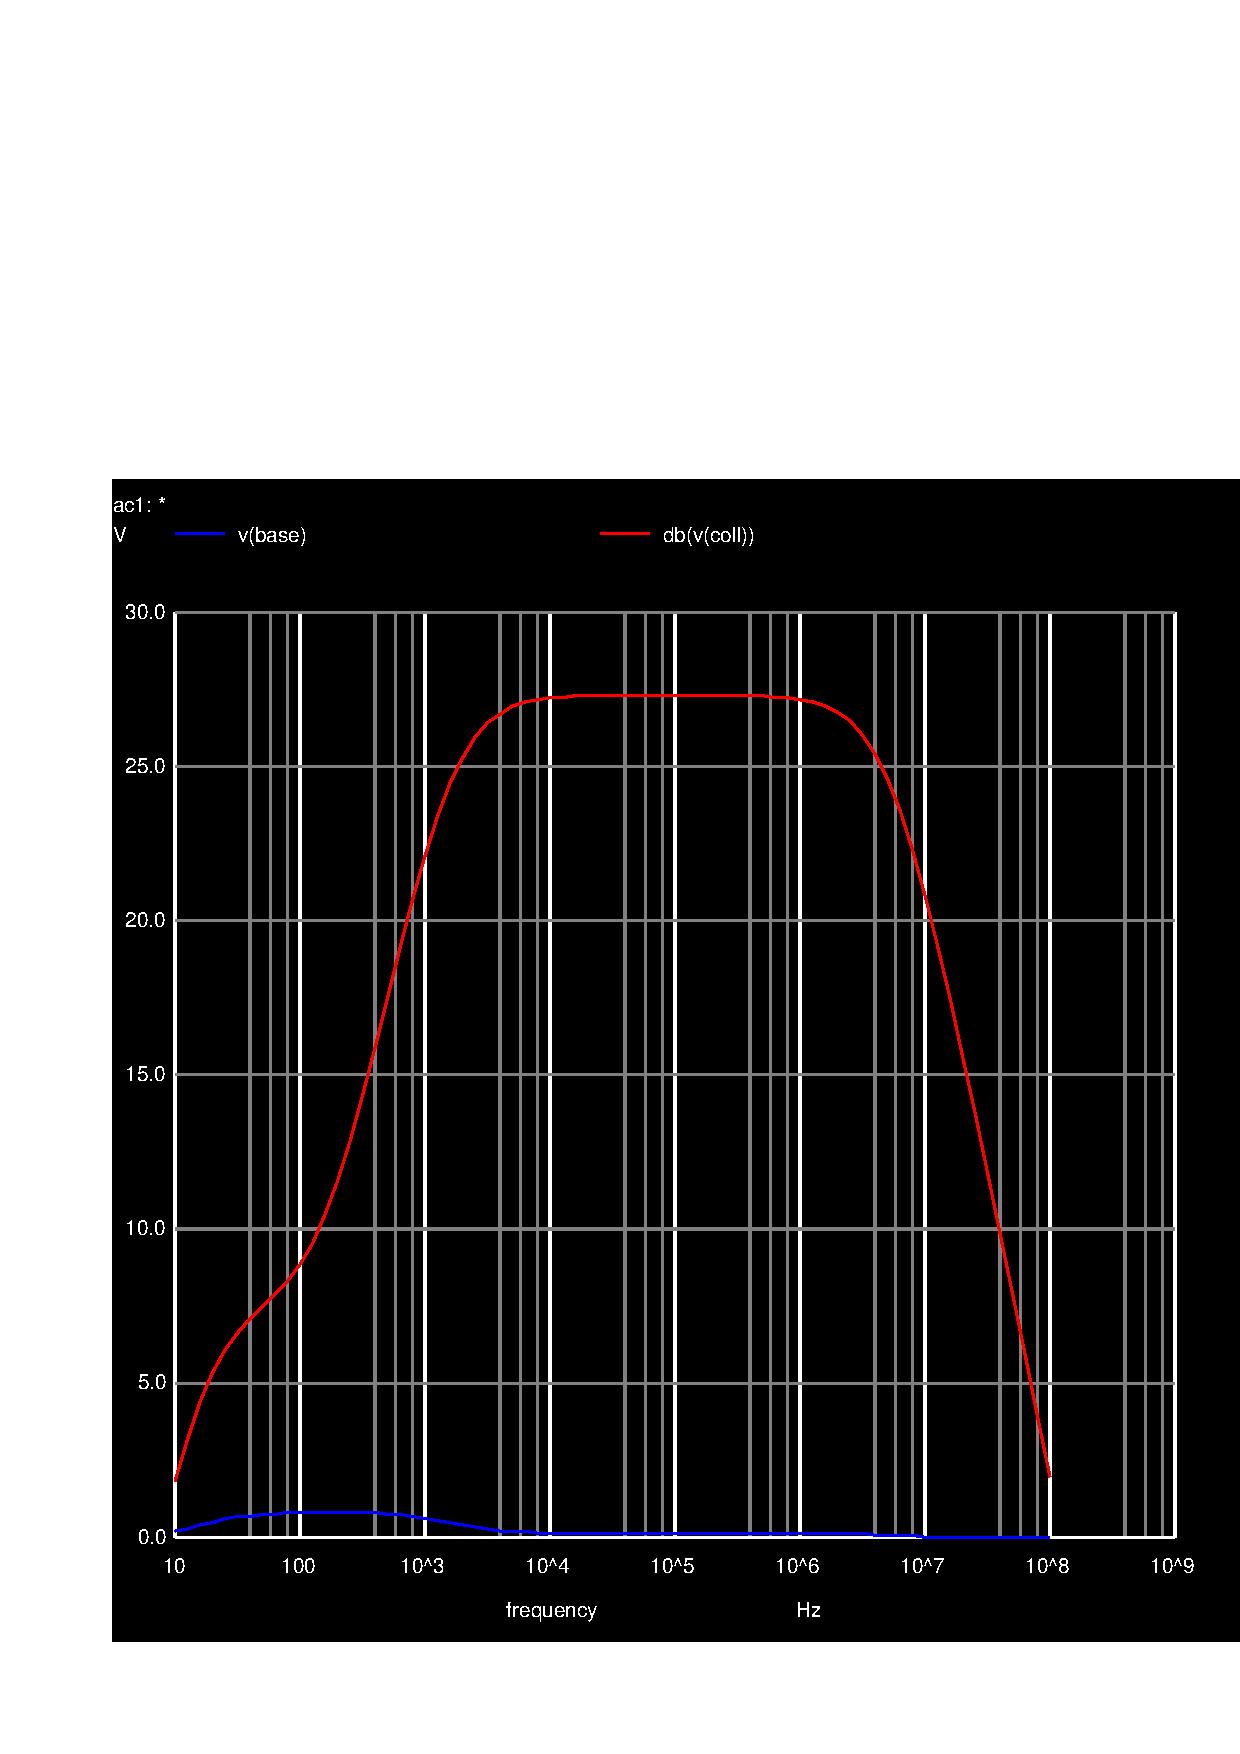
\includegraphics[width=8cm]{../sim/acm.pdf}
\caption{Magnitude graph for $v_6$ and $v_s$.}
\label{fig:magnitude}
\end{figure}







\newpage
\section{Conclusion}
\label{sec:conclusion}
\begin{table}[h!]
  \centering
  \begin{tabular}{|c|c|}
    \hline    
    {\bf Name} & {\bf Value [A or V]} \\ \hline
    @cb[i] & 0.000000e+00\\ \hline
@ce[i] & 0.000000e+00\\ \hline
@q1[ib] & 7.022567e-05\\ \hline
@q1[ic] & 1.404513e-02\\ \hline
@q1[ie] & -1.41154e-02\\ \hline
@q1[is] & 5.765392e-12\\ \hline
@rc[i] & 1.411536e-02\\ \hline
@re[i] & 1.411536e-02\\ \hline
@rf[i] & 7.022567e-05\\ \hline
@rs[i] & 0.000000e+00\\ \hline
v(1) & 0.000000e+00\\ \hline
v(2) & 0.000000e+00\\ \hline
base & 2.254108e+00\\ \hline
coll & 5.765392e+00\\ \hline
emit & 1.411536e+00\\ \hline
vcc & 1.000000e+01\\ \hline

  \end{tabular}
 \begin{tabular}{|c|c|}
 \hline
 \centering
    {\bf Name} & {\bf Value [A or V]} \\ 
    \hline
$I_c$ & 0 \\
$I_b$ & \partialinput{8}{8}{tabela1.tex} \\
$R_1[i]$  & \partialinput{9}{9}{tabela1.tex}\\
$R_2[i]$   & \partialinput{10}{10}{tabela1.tex} \\
$R_3[i]$ & \partialinput{11}{11}{tabela1.tex} \\
$R_4[i]$  & \partialinput{12}{12}{tabela1.tex} \\
$R_5[i]$ & \partialinput{13}{13}{tabela1.tex}\\
$R_6[i]$   & \partialinput{14}{14}{tabela1.tex} \\
$R_7[i]$ & \partialinput{15}{15}{tabela1.tex} \\
$V_1$           & \partialinput{1}{1}{tabela1.tex} \\
$V_2$  & \partialinput{2}{2}{tabela1.tex}\\
$V_3$   & \partialinput{3}{3}{tabela1.tex} \\
$V_5$  & \partialinput{4}{4}{tabela1.tex} \\
$V_6$   & \partialinput{5}{5}{tabela1.tex} \\
$V_7$    & \partialinput{6}{6}{tabela1.tex} \\
$V_8$     &  \partialinput{7}{7}{tabela1.tex}\\
\hline
 \end{tabular}
 \caption{Simulation (right) and Theoretical(left) Node Voltages and Branch currents t < 0.}
  \label{tab:conc1}
\end{table}

\begin{table}[h!]
  \centering
  \begin{tabular}{|c|c|}
    \hline    
    {\bf Name} & {\bf Value [A or V]} \\ \hline
    zout & 7.866317e+00\\ \hline

  \end{tabular}
 \begin{tabular}{|c|c|}
 \hline
 \centering
    {\bf Name} & {\bf Value [A or V]} \\ 
    \hline
$I_b$ & \partialinput{11}{11}{tabela2.tex} \\
$R_1[i]$  & \partialinput{12}{12}{tabela2.tex}\\
$R_2[i]$   & \partialinput{13}{13}{tabela2.tex} \\
$R_3[i]$ & \partialinput{14}{14}{tabela2.tex} \\
$R_4[i]$  & \partialinput{15}{15}{tabela2.tex} \\
$R_5[i]$ & \partialinput{16}{16}{tabela2.tex}\\
$R_6[i]$   & \partialinput{17}{17}{tabela2.tex} \\
$R_7[i]$ & \partialinput{18}{18}{tabela2.tex} \\
$V_1$(t=0)  & 0\\
$V_2$(t=0)  & \partialinput{1}{1}{tabela2.tex}\\
$V_3$(t=0)   & \partialinput{2}{2}{tabela2.tex} \\
$V_5$(t=0)   & \partialinput{3}{3}{tabela2.tex} \\
$V_6$(t=0)    & \partialinput{4}{4}{tabela2.tex} \\
$V_7$(t=0)     & \partialinput{5}{5}{tabela2.tex} \\
$V_8$(t=0)     &  \partialinput{6}{6}{tabela2.tex}\\
\hline
 \end{tabular}
 \caption{Simulation (right) and Theoretical(left) Node Voltages and Branch currents t = 0.}
  \label{tab:conc2}
\end{table}





%\cleardoublepage

% ----------------------------------------------------------------------
%  Bibliography
% ----------------------------------------------------------------------
%\addcontentsline{toc}{section}{\bibname}
%\bibliographystyle{abbrvunsrtnat} % <<<<< SELECT IF USING REFERENCES BY NUMBER (CITATION ORDER)
%\bibliography{../../../BIBfile.bib}

% ----------------------------------------------------------------------
\end{document}
% ----------------------------------------------------------------------

